\documentclass[a4paper,12pt]{article} % добавить leqno в [] для нумерации слева
\usepackage[a4paper,top=1.3cm,bottom=2cm,left=1.5cm,right=1.5cm,marginparwidth=0.75cm]{geometry}
%%% Работа с русским языком
\usepackage{cmap}					% поиск в PDF
\usepackage[warn]{mathtext} 		% русские буквы в фомулах
\usepackage[T2A]{fontenc}			% кодировка
\usepackage[utf8]{inputenc}			% кодировка исходного текста
\usepackage[english,russian]{babel}	% локализация и переносы
\usepackage{physics}
\usepackage{multirow}

%%% Нормальное размещение таблиц (писать [H] в окружении таблицы)
\usepackage{float}
\restylefloat{table}



\usepackage{graphicx}

\usepackage{wrapfig}
\usepackage{tabularx}

\usepackage{hyperref}
\usepackage[rgb]{xcolor}
\hypersetup{
	colorlinks=true,urlcolor=blue
}

\usepackage{pgfplots}
\pgfplotsset{compat=1.9}

%%% Дополнительная работа с математикой
\usepackage{amsmath,amsfonts,amssymb,amsthm,mathtools} % AMS
\usepackage{icomma} % "Умная" запятая: $0,2$ --- число, $0, 2$ --- перечисление

%% Номера формул
\mathtoolsset{showonlyrefs=true} % Показывать номера только у тех формул, на которые есть \eqref{} в тексте.

%% Шрифты
\usepackage{euscript}	 % Шрифт Евклид
\usepackage{mathrsfs} % Красивый матшрифт

%% Свои команды
\DeclareMathOperator{\sgn}{\mathop{sgn}}

%% Перенос знаков в формулах (по Львовскому)
\newcommand*{\hm}[1]{#1\nobreak\discretionary{}
	{\hbox{$\mathsurround=0pt #1$}}{}}

\date{\today}

\usepackage{gensymb}

\begin{document}

\begin{titlepage}
	\begin{center}
		{\large МОСКОВСКИЙ ФИЗИКО-ТЕХНИЧЕСКИЙ ИНСТИТУТ (НАЦИОНАЛЬНЫЙ ИССЛЕДОВАТЕЛЬСКИЙ УНИВЕРСИТЕТ)}
	\end{center}
	\begin{center}
		{\large Физтех-школа физики и исследований им. Ландау}
	\end{center}
	
	
	\vspace{4.5cm}
	{\huge
		\begin{center}
			{\bf Отчёт о выполнении лабораторной работы 2.5.1}\\
			Измерение коэффициента поверхностного натяжения жидкости
		\end{center}
	}
	\vspace{2cm}
	\begin{flushright}
		{\LARGE Автор:\\ Сенокосов Арсений Олегович \\
			\vspace{0.2cm}
			Б02-012}
	\end{flushright}
	\vspace{8cm}
	\begin{center}
		Долгопрудный\\
		\today
	\end{center}
\end{titlepage}


\section{Введение}
\textbf{Цель работы:}  \begin{enumerate}
	\item измерение температурной зависимости  коэффициента поверхностного натяжения дистиллированной воды с использованием известного коэффициента поверхностного натяжения спирта;
	\item определение полной поверхностной энергии  и теплоты, необходимой для изотермического образования единицы  поверхности жидкости  при различной температуре.
\end{enumerate}

\textbf{В работе используются:} прибор  Ребиндера  с термостатом и микроманометром; исследуемые жидкости; стаканы; микроскоп.
\section{Теоретические сведения}

Наличие поверхностного слоя приводит к различию давлений по разные стороны от искривленной границы раздела двух сред.  Для сферического пузырька с воздухом  внутри жидкости избыточное давление даётся формулой Лапласа:

\begin{equation}\label{key}
\Delta P = P_{int} - P_{ext} = \frac{2\sigma}{r},
\end{equation}
где $ \sigma $ -- коэффициент поверхностного натяжения, $ P_{int} $ и $ P_{ext} $ -- давление внутри пузырька и снаружи, $ r $ -- радиус кривизны поверхности раздела двух фаз. Эта формула лежит в основе предлагаемого метода определения коэффициента поверхностного натяжения жидкости. Измеряется давление $ \Delta P $, необходимое для выталкивания в жидкость пузырька воздуха.

\section{Экспериментальная установка}

\begin{figure}[H]
	\begin{center}
		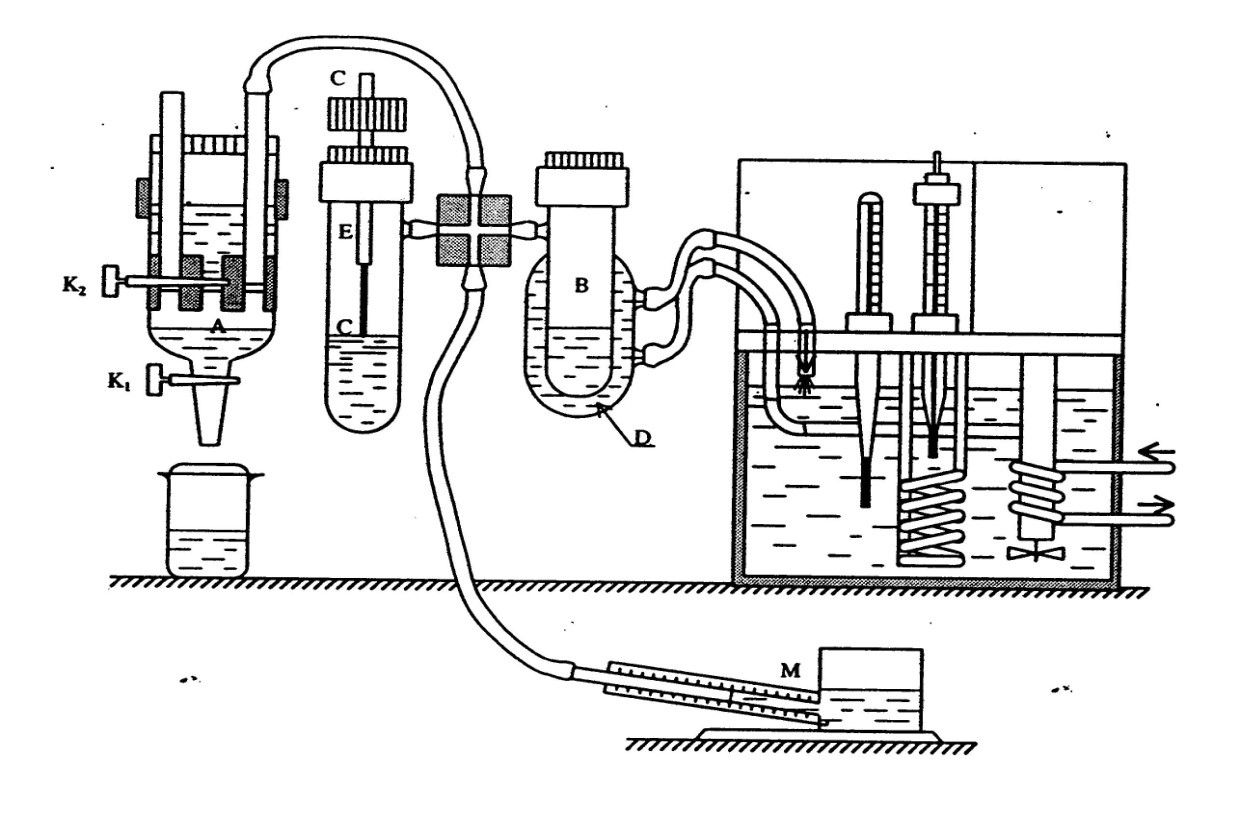
\includegraphics[width=15cm]{ust.jpg}
		\caption{Рисунок экспериментальной установки}\label{img:ust}
	\end{center}
\end{figure}

Исследуемая жидкость (дистиллированная вода) наливается в сосуд (колбу) $ B $ (рис. \ref{img:ust}). Тестовая жидкость  (этиловый спирт) наливается  в сосуд $ E $.  При измерениях  колбы герметично закрываются  пробками. Через одну из двух пробок  проходит полая металлическая игла $ С $. Этой пробкой закрывается сосуд, в котором  проводятся измерения. Верхний конец иглы открыт в атмосферу, а нижний погружен в жидкость. Другой сосуд герметично закрывается второй пробкой. При создании достаточного  разряжения воздуха в колбе с иглой пузырьки воздуха начинают пробулькивать через жидкость. Поверхностное натяжение можно определить по величине разряжения $ \Delta P $ \eqref{key}, необходимого для прохождения пузырьков (при известном радиусе иглы).

Разряжение в системе создается с помощью аспиратора $ A $. Кран $ K_2 $ разделяет две полости аспиратора. Верхняя полость при закрытом кране $ K_2 $ заполняется водой. Затем кран $ K_2 $ открывают и заполняют водой  нижнюю полость  аспиратора.  Разряжение воздуха создается в нижней полости  при открывании крана $ K_1 $, когда  вода вытекает из неё по каплям. В колбах $ В $ и $ С $, соединённых трубками с нижней полостью аспиратора, создается такое же пониженное давление. Разность давлений в полостях с разряженным воздухом и атмосферой измеряется спиртовым микроманометром. 

Для стабилизации температуры исследуемой жидкости через рубашку $ D $ колбы $ В $ непрерывно прогоняется вода из термостата.

Обычно кончик иглы лишь касается поверхности жидкости, чтобы исключить влияние гидростатического давления столба жидкости. Однако при измерении температурной зависимости коэффициента поверхностного натяжения возникает ряд сложностей. Во-первых, большая теплопроводность металлической трубки приводит к тому, что температура на конце трубки заметно ниже, чем в глубине жидкости. Во-вторых, тепловое расширение поднимает уровень жидкости при увеличении температуры.

Обе погрешности можно устранить, погрузив кончик трубки до самого дна. Полное давление, измеренное при этом микроманометром, равно \[ P = \Delta P + \rho g h.\] Заметим, что $ \rho gh $ от температуры практически не зависит, так как подъём уровня жидкости компенсируется уменьшением её плотности (произведение $ \rho g $ определяется массой всей жидкости и поэтому постоянно). Величину  $ \rho g h $ следует измерить двумя способами.

Во-первых, замерить величину $ P_1= \Delta P' $, когда кончик трубки только касается поверхности жидкости. Затем при этой же температуре опустить иглу до дна и замерить $ P_2= \rho gh + \Delta P'' $ ($ \Delta P' $, $ \Delta P'' $ -- давление Лапласа). Из-за  несжимаемости  жидкости можно положить $ \Delta P' = \Delta P'' $ и тогда \[ \rho gh= P_2 - P_1. \]
 
Во-вторых, при измерениях $ P_1 $ и $ P_2 $ замерить линейкой  глубину погружения иглы $ h $. Это можно сделать, замеряя расстояние между верхним концом иглы и любой неподвижной частью прибора при положении иглы на поверхности и в глубине колбы.
\newpage
\section{Ход работы}

\subsection{Измерение диаметра иглы}

Измерим максимальное давление $ \Delta P_{alc} $  при  пробулькивании пузырьков воздуха через спирт. Результаты измерений занесём в таблицу \ref{tab:alcohol}.

\begin{table}[H]
	\centering
	\begin{tabular}{|c|c|c|c|c|}
		\hline
		№ & $ P' $, дел. &  $ P $, Па  & $ \langle P \rangle $, Па   & $ \sigma_{P} $, Па             \\ \hline
		1 & 47  & 92,2 & \multirow{5}{*}{93,1} & \multirow{5}{*}{2,0} \\ \cline{1-3}
		2 & 48  & 94,2 &                       &                      \\ \cline{1-3}
		3 & 48  & 94,2 &                       &                      \\ \cline{1-3}
		4 & 47  & 92,2 &                       &                      \\ \cline{1-3}
		5 & 47  & 92,2 &                       &                      \\ \hline
	\end{tabular}
	\caption{Результаты измерений в спирте}
	\label{tab:alcohol}
\end{table}

Учтём, что показания микроманометра связаны с давлением следующим соотношением: \[ P=P' \cdot 0,2 \cdot 9,81, \] где $ P' $ -- колличество делений шкалы, а константы остаются постоянными во время всей работы и определяются исходя из паспорта устройства.

Вычислим среднее значение измеренного давления. Для этого воспользуемся следующей формулой:

\begin{equation}\label{mid}
\langle P \rangle = \frac{\sum\limits_{k=1}^{N} P_k}{N} \approx 93,1 \text{ Па},
\end{equation}
где $ N $ -- число проведённых измерений.

Также вычислим случайную погрешность измерений по формуле

\begin{equation}\label{occasion}
\sigma_{P}^{\text{случ}} = \sqrt{\frac{1}{N(N-1)}\sum\limits_{k=1}^N\left(P_k-\langle P \rangle\right)^2} \approx 0,5 \text{ Па}.
\end{equation}

Систематическую погрешность определим из расчёта, что погрешность измерения составила $ 1 $ деление прибора, или же \underline{$ \sigma_{P}^\text{сист} \approx 1,9 $ Па}.

Полная погрешность измерений определяется по формуле:

\begin{equation}\label{full_pogr}
\sigma_{P}=\sqrt{(\sigma_{P}^\text{сист})^2 + (\sigma_{P}^\text{случ})^2} \approx 2,0 \text{ Па}.
\end{equation}

Итого получаем \underline{ $ \Delta P_{alc} = (93,1 \pm 2,0) \text{ Па},$} \quad $(\varepsilon = 2,2 \%) $.

\medskip

Согласно ГОСТ 8.428-81 коэффициент поверхностного натяжения этилового спирта при комнатной температуре равен $ \sigma_{alc} = 22,4 $ мН/м. По полученным результатам измерения и при помощи \eqref{key} вычисляем диаметр иглы по формуле:

\label{diametr}

\begin{equation}\label{igla}
d=\frac{4\sigma_{alc}}{\Delta P_{alc}} \approx 0,96 \text{ мм}.
\end{equation}

Также вычисляем погрешность полученного результата:

\begin{equation}\label{igla_pogr}
\sigma_d=d\cdot\varepsilon_{\Delta P_{alc}} \approx 0,02 \text{ мм}.
\end{equation}

Таким образом, получаем окончательный результат измерения диаметра иглы косвенным способом:
\begin{itemize}
	\item $\underline{ d = (0,96 \pm 0,02) \text{ мм},} \: (\varepsilon = 2,2\%). $
\end{itemize}

Также проведём измерение диаметра иглы при помощи оптического микроскопа (см. рис.~\ref{img:igla}).

\begin{figure}[H]
	\begin{center}
		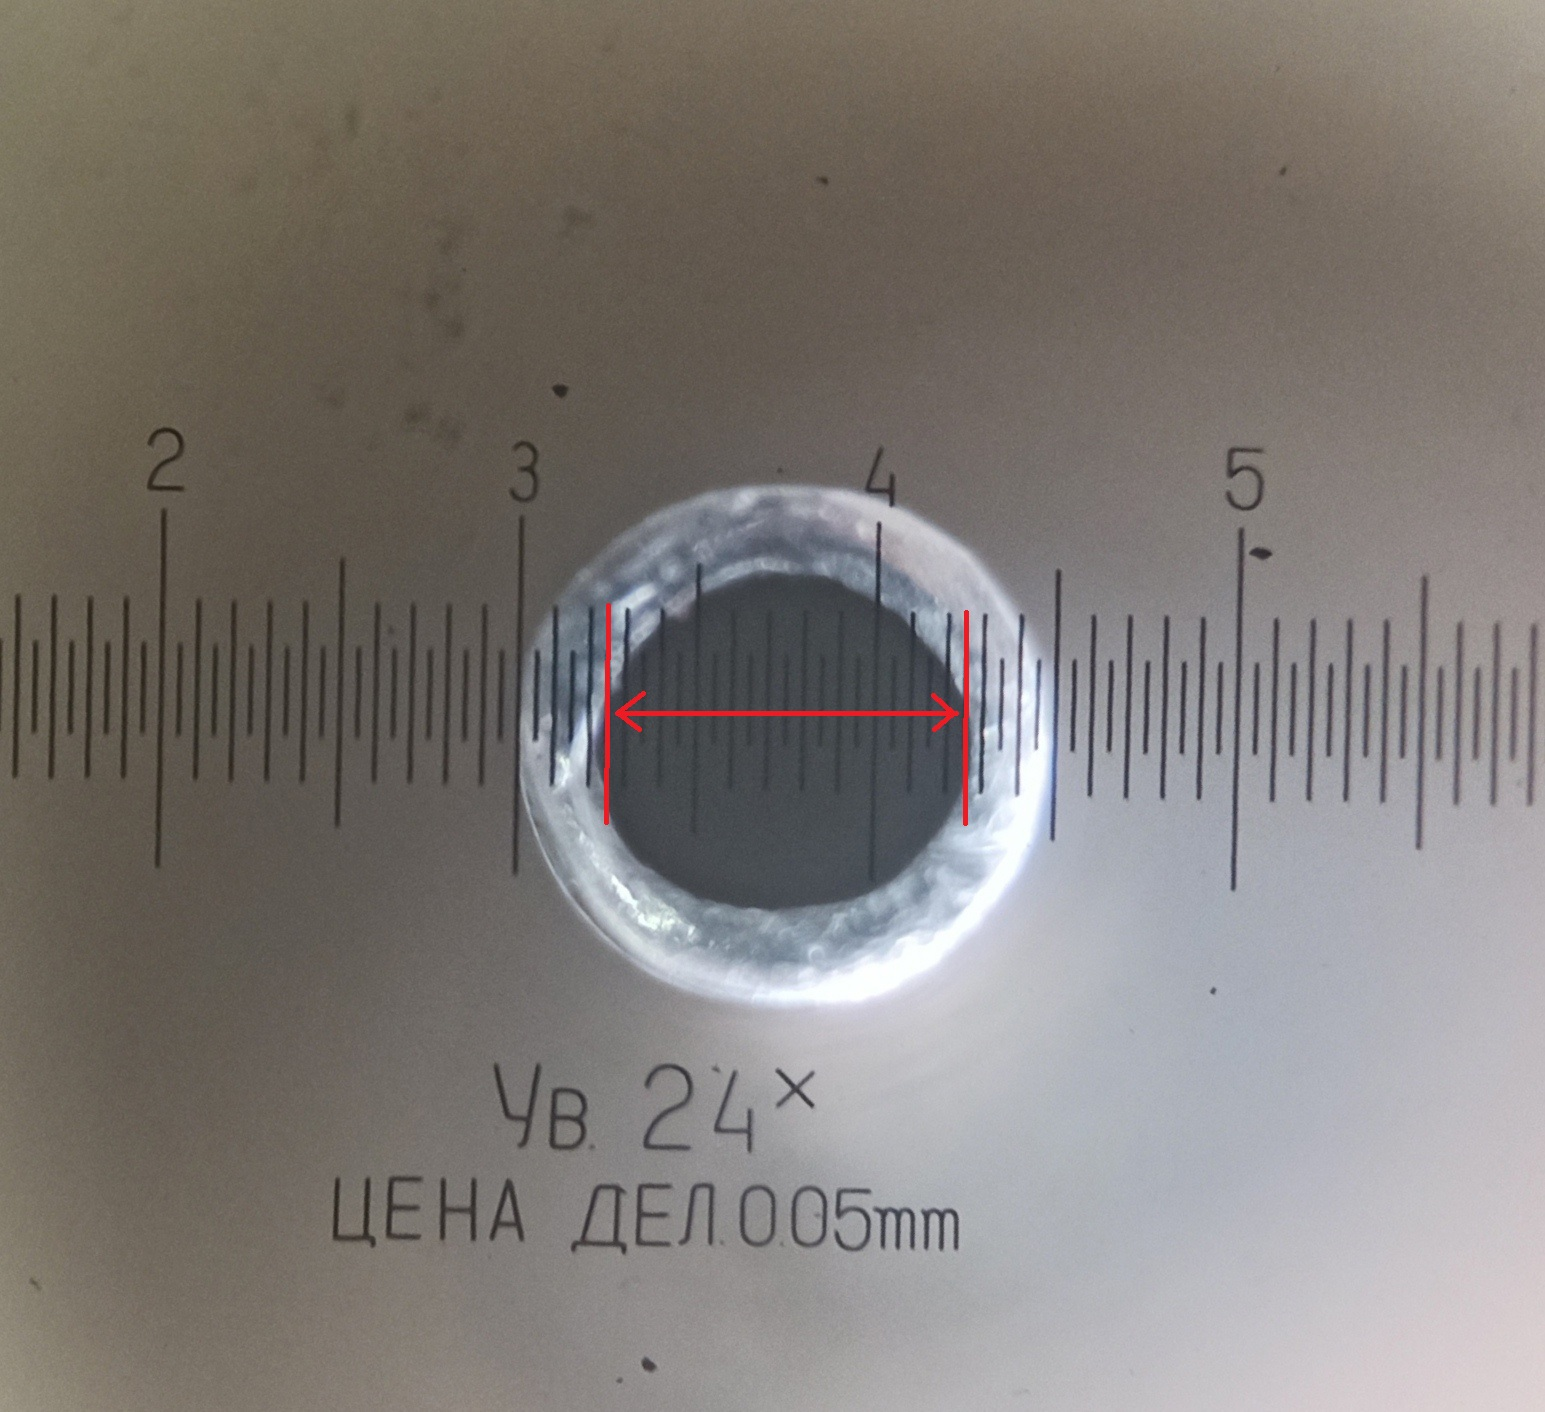
\includegraphics[width=16cm]{igla.jpg}
		\caption{Измерение диаметра иглы}\label{img:igla}
	\end{center}
\end{figure}

По результатам прямого измерения получаем $ \underline{d = (1,00 \pm 0,05) \text{ мм}}, \: (\varepsilon = 5\%) $.

\medskip

Таким образом, диаметр иглы, измеренный двумя различными способами, совпадает в пределах погрешности, что может говорить о справедливости формулы, представленной в теоретических сведениях, а также об исправной работе экспериментальной установки.

\subsection{Определения поправки при измерении давления для погруженной в воду иглы}

Перенесём предварительно промытую и просушенную от спирта иглу в колбу с дистиллированной водой. Измерим максимальное давление $ P_1 $ при пробулькивании пузырьков, когда игла лишь касается поверхности воды. Измерите расстояние между верхним концом иглы и любой неподвижной часть прибора $ h_1 $.

Утопим иглу в воду. Измерим $ h_2 $. Также измерим максимальное давление в пузырьках $ P_2 $. Полученные результаты заносим в таблицу \ref{tab:popravka}.

% Please add the following required packages to your document preamble:
% \usepackage{multirow}
\begin{table}[H]
	\centering
	\begin{tabular}{ccccccc}
		\hline
		\multicolumn{1}{|c|}{№} &
		\multicolumn{1}{c|}{$ P_1 $, дел.} &
		\multicolumn{1}{c|}{$ P_1 $, Па} &
		\multicolumn{1}{c|}{$ \langle P_1 \rangle $, Па} &
		\multicolumn{1}{c|}{$ \sigma_{P_1} $, Па} &
		\multicolumn{1}{c|}{$ h_1 $, мм} &
		\multicolumn{1}{c|}{$ \sigma_{h_1} $, мм} \\ \hline
		\multicolumn{1}{|c|}{1} &
		\multicolumn{1}{c|}{131} &
		\multicolumn{1}{c|}{257,0} &
		\multicolumn{1}{c|}{\multirow{6}{*}{257,0}} &
		\multicolumn{1}{c|}{\multirow{6}{*}{1,9}} &
		\multicolumn{1}{c|}{\multirow{6}{*}{54,0}} &
		\multicolumn{1}{c|}{\multirow{6}{*}{0,5}} \\ \cline{1-3}
		\multicolumn{1}{|c|}{2} &
		\multicolumn{1}{c|}{131} &
		\multicolumn{1}{c|}{257,0} &
		\multicolumn{1}{c|}{} &
		\multicolumn{1}{c|}{} &
		\multicolumn{1}{c|}{} &
		\multicolumn{1}{c|}{} \\ \cline{1-3}
		\multicolumn{1}{|c|}{3} &
		\multicolumn{1}{c|}{131} &
		\multicolumn{1}{c|}{257,0} &
		\multicolumn{1}{c|}{} &
		\multicolumn{1}{c|}{} &
		\multicolumn{1}{c|}{} &
		\multicolumn{1}{c|}{} \\ \cline{1-3}
		\multicolumn{1}{|c|}{4} &
		\multicolumn{1}{c|}{131} &
		\multicolumn{1}{c|}{257,0} &
		\multicolumn{1}{c|}{} &
		\multicolumn{1}{c|}{} &
		\multicolumn{1}{c|}{} &
		\multicolumn{1}{c|}{} \\ \cline{1-3}
		\multicolumn{1}{|c|}{5} &
		\multicolumn{1}{c|}{131} &
		\multicolumn{1}{c|}{257,0} &
		\multicolumn{1}{c|}{} &
		\multicolumn{1}{c|}{} &
		\multicolumn{1}{c|}{} &
		\multicolumn{1}{c|}{} \\ \cline{1-3}
		\multicolumn{1}{|c|}{6} &
		\multicolumn{1}{c|}{131} &
		\multicolumn{1}{c|}{257,0} &
		\multicolumn{1}{c|}{} &
		\multicolumn{1}{c|}{} &
		\multicolumn{1}{c|}{} &
		\multicolumn{1}{c|}{} \\ \hline
		&
		&
		&
		&
		&
		&
		\\ \hline
		\multicolumn{1}{|c|}{№} &
		\multicolumn{1}{c|}{$ P_2 $, дел.} &
		\multicolumn{1}{c|}{$ P_2 $, Па} &
		\multicolumn{1}{c|}{$ \langle P_2 \rangle $, Па} &
		\multicolumn{1}{c|}{$ \sigma_{P_2} $, Па} &
		\multicolumn{1}{c|}{$ h_2 $, мм} &
		\multicolumn{1}{c|}{$ \sigma_{h_2} $, мм} \\ \hline
		\multicolumn{1}{|c|}{1} &
		\multicolumn{1}{c|}{190} &
		\multicolumn{1}{c|}{372,2} &
		\multicolumn{1}{c|}{\multirow{6}{*}{374,4}} &
		\multicolumn{1}{c|}{\multirow{6}{*}{1,9}} &
		\multicolumn{1}{c|}{\multirow{6}{*}{42,0}} &
		\multicolumn{1}{c|}{\multirow{6}{*}{0,5}} \\ \cline{1-3}
		\multicolumn{1}{|c|}{2} &
		\multicolumn{1}{c|}{191} &
		\multicolumn{1}{c|}{374,7} &
		\multicolumn{1}{c|}{} &
		\multicolumn{1}{c|}{} &
		\multicolumn{1}{c|}{} &
		\multicolumn{1}{c|}{} \\ \cline{1-3}
		\multicolumn{1}{|c|}{3} &
		\multicolumn{1}{c|}{191} &
		\multicolumn{1}{c|}{374,7} &
		\multicolumn{1}{c|}{} &
		\multicolumn{1}{c|}{} &
		\multicolumn{1}{c|}{} &
		\multicolumn{1}{c|}{} \\ \cline{1-3}
		\multicolumn{1}{|c|}{4} &
		\multicolumn{1}{c|}{191} &
		\multicolumn{1}{c|}{374,7} &
		\multicolumn{1}{c|}{} &
		\multicolumn{1}{c|}{} &
		\multicolumn{1}{c|}{} &
		\multicolumn{1}{c|}{} \\ \cline{1-3}
		\multicolumn{1}{|c|}{5} &
		\multicolumn{1}{c|}{191} &
		\multicolumn{1}{c|}{374,7} &
		\multicolumn{1}{c|}{} &
		\multicolumn{1}{c|}{} &
		\multicolumn{1}{c|}{} &
		\multicolumn{1}{c|}{} \\ \cline{1-3}
		\multicolumn{1}{|c|}{6} &
		\multicolumn{1}{c|}{191} &
		\multicolumn{1}{c|}{374,7} &
		\multicolumn{1}{c|}{} &
		\multicolumn{1}{c|}{} &
		\multicolumn{1}{c|}{} &
		\multicolumn{1}{c|}{} \\ \hline
	\end{tabular}
	\caption{Определение поправки к давлению}
	\label{tab:popravka}
\end{table}

Исходя из экспериментальных данных, определяем среднее значение давления $ \langle P \rangle $ и погрешность измерения $ \sigma_{P} $ по формулам \eqref{mid}, \eqref{occasion} и \eqref{full_pogr}.

По полученным данным определяем \[ P_2-P_1 = 117,4 \text{ Па}. \]

Также вычисляем погрешность:  \begin{equation}\label{pogr_sum}
\sigma_{\Delta P} = \sqrt{\sigma^2_{P_1}+\sigma^2_{P_2}} \approx 2,8 \text{ Па}.
\end{equation}

Таким образом, получаем $ \underline{\Delta P = (117,4 \pm 2,8) \text{ Па},} \: (\varepsilon = 2,4\%).$

По полученному значению $ \Delta P $ можем рассчитать $ \Delta h $ по следующей формуле: \[ \Delta h = \frac{\Delta P}{\rho g} \approx 11,9 \text{ мм}, \] где $ \rho = 1000 $ кг/$ \text{м}^3 $ -- плотность воды и $ g = 9,81 $ м/$ \text{с}^2 $ -- ускорение свободного падения.

\medskip

При этом погрешность нашего измерения равна \[ \sigma_{\Delta h} = \Delta h \cdot \varepsilon_{\Delta P} \approx 0,3 \text{ мм}. \]

Таким образом, получаем $ \underline{\Delta h = (11,9 \pm 0,3) \text{ мм}}, \: (\varepsilon = 2,4\%). $

\medskip

Заметим, что полученный результат в пределах погрешности совпадает с результатом, полученном прямым измерением $ \underline{\Delta h' = (12,0 \pm 0,7) \text{ мм},} \: (\varepsilon = 5,9\%). $

Значит, в ходе дальнейших измерений мы будем делать поправку \label{popravka} $  \underline{\Delta P = (117,4 \pm 2,8) \text{ Па},}$ на~добавочное давление со стороны столба жидкости.

\subsection{Измерение температурной зависимости коэффициента поверхностного натяжения}

Снимем температурную зависимость $ \sigma(T) $ дистиллированной воды. Для этого включим термостат и подождём, пока нужная нам температура не стабилизируется. После этого проведём измерение давления. Для уменьшения погрешности опыта замер давления  при фиксированной температуре проведём несколько раз. Результаты измерений занесём в таблицу \ref{tab:pov}.

% Please add the following required packages to your document preamble:
% \usepackage{multirow}
\begin{table}[H]
	\centering
	\begin{tabular}{ccccccc}
		\hline
		\multicolumn{1}{|c|}{$ T $, К} &
		\multicolumn{1}{c|}{$ P' $, дел} &
		\multicolumn{1}{c|}{$ P' $, Па} &
		\multicolumn{1}{c|}{$ \langle P' \rangle $, Па} &
		\multicolumn{1}{c|}{$ \sigma_{P'} $, Па} &
		\multicolumn{1}{c|}{$ P $, Па} &
		\multicolumn{1}{c|}{$ \sigma_P $, Па} \\ \hline
		\multicolumn{1}{|c|}{\multirow{5}{*}{302}} &
		\multicolumn{1}{c|}{190} &
		\multicolumn{1}{c|}{372,8} &
		\multicolumn{1}{c|}{\multirow{5}{*}{374,3}} &
		\multicolumn{1}{c|}{\multirow{5}{*}{2,0}} &
		\multicolumn{1}{c|}{\multirow{5}{*}{257,0}} &
		\multicolumn{1}{c|}{\multirow{5}{*}{3,4}} \\ \cline{2-3}
		\multicolumn{1}{|c|}{} &
		\multicolumn{1}{c|}{191} &
		\multicolumn{1}{c|}{374,7} &
		\multicolumn{1}{c|}{} &
		\multicolumn{1}{c|}{} &
		\multicolumn{1}{c|}{} &
		\multicolumn{1}{c|}{} \\ \cline{2-3}
		\multicolumn{1}{|c|}{} &
		\multicolumn{1}{c|}{191} &
		\multicolumn{1}{c|}{374,7} &
		\multicolumn{1}{c|}{} &
		\multicolumn{1}{c|}{} &
		\multicolumn{1}{c|}{} &
		\multicolumn{1}{c|}{} \\ \cline{2-3}
		\multicolumn{1}{|c|}{} &
		\multicolumn{1}{c|}{191} &
		\multicolumn{1}{c|}{374,7} &
		\multicolumn{1}{c|}{} &
		\multicolumn{1}{c|}{} &
		\multicolumn{1}{c|}{} &
		\multicolumn{1}{c|}{} \\ \cline{2-3}
		\multicolumn{1}{|c|}{} &
		\multicolumn{1}{c|}{191} &
		\multicolumn{1}{c|}{374,7} &
		\multicolumn{1}{c|}{} &
		\multicolumn{1}{c|}{} &
		\multicolumn{1}{c|}{} &
		\multicolumn{1}{c|}{} \\ \hline
		&
		&
		&
		&
		&
		&
		\\ \hline
		\multicolumn{1}{|c|}{$ T $, К} &
		\multicolumn{1}{c|}{$ P' $, дел} &
		\multicolumn{1}{c|}{$ P' $, Па} &
		\multicolumn{1}{c|}{$ \langle P' \rangle $, Па} &
		\multicolumn{1}{c|}{$ \sigma_{P'} $, Па} &
		\multicolumn{1}{c|}{$ P $, Па} &
		\multicolumn{1}{c|}{$ \sigma_P $, Па} \\ \hline
		\multicolumn{1}{|c|}{\multirow{5}{*}{307}} &
		\multicolumn{1}{c|}{189} &
		\multicolumn{1}{c|}{370,8} &
		\multicolumn{1}{c|}{\multirow{5}{*}{370,8}} &
		\multicolumn{1}{c|}{\multirow{5}{*}{2,0}} &
		\multicolumn{1}{c|}{\multirow{5}{*}{253,4}} &
		\multicolumn{1}{c|}{\multirow{5}{*}{3,4}} \\ \cline{2-3}
		\multicolumn{1}{|c|}{} &
		\multicolumn{1}{c|}{189} &
		\multicolumn{1}{c|}{370,8} &
		\multicolumn{1}{c|}{} &
		\multicolumn{1}{c|}{} &
		\multicolumn{1}{c|}{} &
		\multicolumn{1}{c|}{} \\ \cline{2-3}
		\multicolumn{1}{|c|}{} &
		\multicolumn{1}{c|}{189} &
		\multicolumn{1}{c|}{370,8} &
		\multicolumn{1}{c|}{} &
		\multicolumn{1}{c|}{} &
		\multicolumn{1}{c|}{} &
		\multicolumn{1}{c|}{} \\ \cline{2-3}
		\multicolumn{1}{|c|}{} &
		\multicolumn{1}{c|}{189} &
		\multicolumn{1}{c|}{370,8} &
		\multicolumn{1}{c|}{} &
		\multicolumn{1}{c|}{} &
		\multicolumn{1}{c|}{} &
		\multicolumn{1}{c|}{} \\ \cline{2-3}
		\multicolumn{1}{|c|}{} &
		\multicolumn{1}{c|}{189} &
		\multicolumn{1}{c|}{370,8} &
		\multicolumn{1}{c|}{} &
		\multicolumn{1}{c|}{} &
		\multicolumn{1}{c|}{} &
		\multicolumn{1}{c|}{} \\ \hline
		&
		&
		&
		&
		&
		&
		\\ \hline
		\multicolumn{1}{|c|}{$ T $, К} &
		\multicolumn{1}{c|}{$ P' $, дел} &
		\multicolumn{1}{c|}{$ P' $, Па} &
		\multicolumn{1}{c|}{$ \langle P' \rangle $, Па} &
		\multicolumn{1}{c|}{$ \sigma_{P'} $, Па} &
		\multicolumn{1}{c|}{$ P $, Па} &
		\multicolumn{1}{c|}{$ \sigma_P $, Па} \\ \hline
		\multicolumn{1}{|c|}{\multirow{5}{*}{312}} &
		\multicolumn{1}{c|}{187} &
		\multicolumn{1}{c|}{366,9} &
		\multicolumn{1}{c|}{\multirow{5}{*}{366,9}} &
		\multicolumn{1}{c|}{\multirow{5}{*}{2,0}} &
		\multicolumn{1}{c|}{\multirow{5}{*}{249,5}} &
		\multicolumn{1}{c|}{\multirow{5}{*}{3,4}} \\ \cline{2-3}
		\multicolumn{1}{|c|}{} &
		\multicolumn{1}{c|}{187} &
		\multicolumn{1}{c|}{366,9} &
		\multicolumn{1}{c|}{} &
		\multicolumn{1}{c|}{} &
		\multicolumn{1}{c|}{} &
		\multicolumn{1}{c|}{} \\ \cline{2-3}
		\multicolumn{1}{|c|}{} &
		\multicolumn{1}{c|}{187} &
		\multicolumn{1}{c|}{366,9} &
		\multicolumn{1}{c|}{} &
		\multicolumn{1}{c|}{} &
		\multicolumn{1}{c|}{} &
		\multicolumn{1}{c|}{} \\ \cline{2-3}
		\multicolumn{1}{|c|}{} &
		\multicolumn{1}{c|}{187} &
		\multicolumn{1}{c|}{366,9} &
		\multicolumn{1}{c|}{} &
		\multicolumn{1}{c|}{} &
		\multicolumn{1}{c|}{} &
		\multicolumn{1}{c|}{} \\ \cline{2-3}
		\multicolumn{1}{|c|}{} &
		\multicolumn{1}{c|}{187} &
		\multicolumn{1}{c|}{366,9} &
		\multicolumn{1}{c|}{} &
		\multicolumn{1}{c|}{} &
		\multicolumn{1}{c|}{} &
		\multicolumn{1}{c|}{} \\ \hline
		&
		&
		&
		&
		&
		&
		\\ \hline
		\multicolumn{1}{|c|}{$ T $, К} &
		\multicolumn{1}{c|}{$ P' $, дел} &
		\multicolumn{1}{c|}{$ P' $, Па} &
		\multicolumn{1}{c|}{$ \langle P' \rangle $, Па} &
		\multicolumn{1}{c|}{$ \sigma_{P'} $, Па} &
		\multicolumn{1}{c|}{$ P $, Па} &
		\multicolumn{1}{c|}{$ \sigma_P $, Па} \\ \hline
		\multicolumn{1}{|c|}{\multirow{5}{*}{317}} &
		\multicolumn{1}{c|}{185} &
		\multicolumn{1}{c|}{363,0} &
		\multicolumn{1}{c|}{\multirow{5}{*}{363,4}} &
		\multicolumn{1}{c|}{\multirow{5}{*}{2,0}} &
		\multicolumn{1}{c|}{\multirow{5}{*}{246,0}} &
		\multicolumn{1}{c|}{\multirow{5}{*}{3,4}} \\ \cline{2-3}
		\multicolumn{1}{|c|}{} &
		\multicolumn{1}{c|}{185} &
		\multicolumn{1}{c|}{363,0} &
		\multicolumn{1}{c|}{} &
		\multicolumn{1}{c|}{} &
		\multicolumn{1}{c|}{} &
		\multicolumn{1}{c|}{} \\ \cline{2-3}
		\multicolumn{1}{|c|}{} &
		\multicolumn{1}{c|}{186} &
		\multicolumn{1}{c|}{364,9} &
		\multicolumn{1}{c|}{} &
		\multicolumn{1}{c|}{} &
		\multicolumn{1}{c|}{} &
		\multicolumn{1}{c|}{} \\ \cline{2-3}
		\multicolumn{1}{|c|}{} &
		\multicolumn{1}{c|}{185} &
		\multicolumn{1}{c|}{363,0} &
		\multicolumn{1}{c|}{} &
		\multicolumn{1}{c|}{} &
		\multicolumn{1}{c|}{} &
		\multicolumn{1}{c|}{} \\ \cline{2-3}
		\multicolumn{1}{|c|}{} &
		\multicolumn{1}{c|}{185} &
		\multicolumn{1}{c|}{363,0} &
		\multicolumn{1}{c|}{} &
		\multicolumn{1}{c|}{} &
		\multicolumn{1}{c|}{} &
		\multicolumn{1}{c|}{} \\ \hline
		&
		&
		&
		&
		&
		&
		\\ \hline
		\multicolumn{1}{|c|}{$ T $, К} &
		\multicolumn{1}{c|}{$ P' $, дел} &
		\multicolumn{1}{c|}{$ P' $, Па} &
		\multicolumn{1}{c|}{$ \langle P' \rangle $, Па} &
		\multicolumn{1}{c|}{$ \sigma_{P'} $, Па} &
		\multicolumn{1}{c|}{$ P $, Па} &
		\multicolumn{1}{c|}{$ \sigma_P $, Па} \\ \hline
		\multicolumn{1}{|c|}{\multirow{5}{*}{322}} &
		\multicolumn{1}{c|}{184} &
		\multicolumn{1}{c|}{361,0} &
		\multicolumn{1}{c|}{\multirow{5}{*}{360,6}} &
		\multicolumn{1}{c|}{\multirow{5}{*}{2,0}} &
		\multicolumn{1}{c|}{\multirow{5}{*}{243,2}} &
		\multicolumn{1}{c|}{\multirow{5}{*}{3,4}} \\ \cline{2-3}
		\multicolumn{1}{|c|}{} &
		\multicolumn{1}{c|}{184} &
		\multicolumn{1}{c|}{361,0} &
		\multicolumn{1}{c|}{} &
		\multicolumn{1}{c|}{} &
		\multicolumn{1}{c|}{} &
		\multicolumn{1}{c|}{} \\ \cline{2-3}
		\multicolumn{1}{|c|}{} &
		\multicolumn{1}{c|}{183} &
		\multicolumn{1}{c|}{359,0} &
		\multicolumn{1}{c|}{} &
		\multicolumn{1}{c|}{} &
		\multicolumn{1}{c|}{} &
		\multicolumn{1}{c|}{} \\ \cline{2-3}
		\multicolumn{1}{|c|}{} &
		\multicolumn{1}{c|}{184} &
		\multicolumn{1}{c|}{361,0} &
		\multicolumn{1}{c|}{} &
		\multicolumn{1}{c|}{} &
		\multicolumn{1}{c|}{} &
		\multicolumn{1}{c|}{} \\ \cline{2-3}
		\multicolumn{1}{|c|}{} &
		\multicolumn{1}{c|}{184} &
		\multicolumn{1}{c|}{361,0} &
		\multicolumn{1}{c|}{} &
		\multicolumn{1}{c|}{} &
		\multicolumn{1}{c|}{} &
		\multicolumn{1}{c|}{} \\ \hline
		&
		&
		&
		&
		&
		&
		\\ \hline
		\multicolumn{1}{|c|}{$ T $, К} &
		\multicolumn{1}{c|}{$ P' $, дел} &
		\multicolumn{1}{c|}{$ P' $, Па} &
		\multicolumn{1}{c|}{$ \langle P' \rangle $, Па} &
		\multicolumn{1}{c|}{$ \sigma_{P'} $, Па} &
		\multicolumn{1}{c|}{$ P $, Па} &
		\multicolumn{1}{c|}{$ \sigma_P $, Па} \\ \hline
		\multicolumn{1}{|c|}{\multirow{5}{*}{327}} &
		\multicolumn{1}{c|}{183} &
		\multicolumn{1}{c|}{359,0} &
		\multicolumn{1}{c|}{\multirow{5}{*}{358,3}} &
		\multicolumn{1}{c|}{\multirow{5}{*}{2,0}} &
		\multicolumn{1}{c|}{\multirow{5}{*}{240,9}} &
		\multicolumn{1}{c|}{\multirow{5}{*}{3,4}} \\ \cline{2-3}
		\multicolumn{1}{|c|}{} &
		\multicolumn{1}{c|}{182} &
		\multicolumn{1}{c|}{357,1} &
		\multicolumn{1}{c|}{} &
		\multicolumn{1}{c|}{} &
		\multicolumn{1}{c|}{} &
		\multicolumn{1}{c|}{} \\ \cline{2-3}
		\multicolumn{1}{|c|}{} &
		\multicolumn{1}{c|}{183} &
		\multicolumn{1}{c|}{359,0} &
		\multicolumn{1}{c|}{} &
		\multicolumn{1}{c|}{} &
		\multicolumn{1}{c|}{} &
		\multicolumn{1}{c|}{} \\ \cline{2-3}
		\multicolumn{1}{|c|}{} &
		\multicolumn{1}{c|}{183} &
		\multicolumn{1}{c|}{359,0} &
		\multicolumn{1}{c|}{} &
		\multicolumn{1}{c|}{} &
		\multicolumn{1}{c|}{} &
		\multicolumn{1}{c|}{} \\ \cline{2-3}
		\multicolumn{1}{|c|}{} &
		\multicolumn{1}{c|}{182} &
		\multicolumn{1}{c|}{357,1} &
		\multicolumn{1}{c|}{} &
		\multicolumn{1}{c|}{} &
		\multicolumn{1}{c|}{} &
		\multicolumn{1}{c|}{} \\ \hline
		&
		&
		&
		&
		&
		&
		\\ \hline
		\multicolumn{1}{|c|}{$ T $, К} &
		\multicolumn{1}{c|}{$ P' $, дел} &
		\multicolumn{1}{c|}{$ P' $, Па} &
		\multicolumn{1}{c|}{$ \langle P' \rangle $, Па} &
		\multicolumn{1}{c|}{$ \sigma_{P'} $, Па} &
		\multicolumn{1}{c|}{$ P $, Па} &
		\multicolumn{1}{c|}{$ \sigma_P $, Па} \\ \hline
		\multicolumn{1}{|c|}{\multirow{5}{*}{332}} &
		\multicolumn{1}{c|}{181} &
		\multicolumn{1}{c|}{355,1} &
		\multicolumn{1}{c|}{\multirow{5}{*}{354,7}} &
		\multicolumn{1}{c|}{\multirow{5}{*}{2,0}} &
		\multicolumn{1}{c|}{\multirow{5}{*}{237,3}} &
		\multicolumn{1}{c|}{\multirow{5}{*}{3,4}} \\ \cline{2-3}
		\multicolumn{1}{|c|}{} &
		\multicolumn{1}{c|}{181} &
		\multicolumn{1}{c|}{355,1} &
		\multicolumn{1}{c|}{} &
		\multicolumn{1}{c|}{} &
		\multicolumn{1}{c|}{} &
		\multicolumn{1}{c|}{} \\ \cline{2-3}
		\multicolumn{1}{|c|}{} &
		\multicolumn{1}{c|}{181} &
		\multicolumn{1}{c|}{355,1} &
		\multicolumn{1}{c|}{} &
		\multicolumn{1}{c|}{} &
		\multicolumn{1}{c|}{} &
		\multicolumn{1}{c|}{} \\ \cline{2-3}
		\multicolumn{1}{|c|}{} &
		\multicolumn{1}{c|}{181} &
		\multicolumn{1}{c|}{355,1} &
		\multicolumn{1}{c|}{} &
		\multicolumn{1}{c|}{} &
		\multicolumn{1}{c|}{} &
		\multicolumn{1}{c|}{} \\ \cline{2-3}
		\multicolumn{1}{|c|}{} &
		\multicolumn{1}{c|}{180} &
		\multicolumn{1}{c|}{353,2} &
		\multicolumn{1}{c|}{} &
		\multicolumn{1}{c|}{} &
		\multicolumn{1}{c|}{} &
		\multicolumn{1}{c|}{} \\ \hline
	\end{tabular}
	\caption{Измерение температурной зависимости коэффициента поверхностного натяжения}
	\label{tab:pov}
\end{table}
\newpage
Исходя из экспериментальных данных, определяем среднее значение давления $ \langle P' \rangle $ и погрешность измерения $ \sigma_{P'} $ (для давления без учёта поправки) по формулам \eqref{mid}, \eqref{occasion} и \eqref{full_pogr}.

Также учитываем поправку к измеренному давлению, которая была вычислена в \ref{popravka}. Погрешность после её учёта вычисляем по формуле \eqref{pogr_sum}. Полученные результаты также заносим в таблицу \ref{tab:pov}.

По полученным данным вычислим коэффициент поверхностного натяжения для каждой из температур по формуле

\begin{equation}\label{sigma}
\sigma = \frac{Pd}{4},
\end{equation}
где $ d $ -- диаметр иглы, вычисленный в \ref{diametr}. Погрешность такого результата вычисляется по следующей формуле:

\begin{equation}\label{otn_pogr}
\sigma_\sigma = \sigma\sqrt{\varepsilon^2_P + \varepsilon^2_d}.
\end{equation}

Полученные результаты заносим в таблицу \ref{tab:temp}.

\begin{table}[H]
	\centering
	\begin{tabular}{|c|c|c|c|c|}
		\hline
		№ & $ T $, К   & $ \sigma_T, К $   & $ \sigma $, мН/м & $ \sigma_\sigma $, мН/м \\ \hline
		1 & 302,0 & 0,1 & 61,9  & 1,6   \\ \hline
		2 & 307,0 & 0,1 & 61,0  & 1,6   \\ \hline
		3 & 312,0 & 0,1 & 60,1  & 1,5   \\ \hline
		4 & 317,0 & 0,1 & 59,2  & 1,5   \\ \hline
		5 & 322,0 & 0,1 & 58,6  & 1,5   \\ \hline
		6 & 327,0 & 0,1 & 58,0  & 1,5   \\ \hline
		7 & 332,0 & 0,1 & 57,2  & 1,5   \\ \hline
	\end{tabular}
	\caption{Зависимость коэффициента пов. натяжения от $T$}
	\label{tab:temp}
\end{table}

Полученную зависимость наносим на график (рис. ). Вычислим коэффициенты аппроксимирующей прямой $ \sigma = kT + b $, где $ \displaystyle k = \frac{d\sigma}{dT} $, используя метод наименьших квадратов:

\[ k = \frac{\langle T\sigma \rangle - \langle T \rangle \langle \sigma \rangle}{\langle T^2 \rangle - \langle T \rangle ^2} \approx -0,155\text{ } \frac{\text{мН}}{\text{м}\cdot\text{К}},\]

\[ b = \langle \sigma \rangle - k\langle T \rangle \approx 108,6\text{ } \frac{\text{мН}}{\text{м}}. \]

Случайные погрешности определения этих коэффициентов вычислим по следующим формулам:

\[ \sigma^\text{случ}_k = \sqrt{\frac{1}{N-2} \left(\frac{\left\langle\left(\sigma - \langle \sigma\right\rangle\right)^2 \rangle}{\left\langle\left(T - \langle T\right\rangle\right)^2 \rangle}\right)-k^2} \approx 0,005 \text{ } \frac{\text{мН}}{\text{м}\cdot\text{К}},\]

\[ \sigma^\text{случ}_b=\sigma^\text{случ}_k\sqrt{\left\langle x^2 \right\rangle} \approx 1,7\text{ } \frac{\text{мН}}{\text{м}}. \]

Систематические погрешности оценим по следующим формулам:

\[ \sigma^\text{сист}_k = |k|\sqrt{\varepsilon^2_T+\varepsilon^2_\sigma} \approx 0,004 \text{ } \frac{\text{мН}}{\text{м}\cdot\text{К}}, \]
\[ \sigma^\text{сист}_b = |b|\sqrt{\varepsilon^2_T+\varepsilon^2_\sigma} \approx 2,8 \text{ } \frac{\text{мН}}{\text{м}}. \]

\newpage

Таким образом, полные погрешности измерений определяются следующими соотношениями:
\[ \sigma_k = \sqrt{(\sigma_k^\text{сист})^2 + (\sigma_k^\text{случ})^2} \approx 0,006 \text{ } \frac{\text{мН}}{\text{м}\cdot\text{К}},\]
\[ \sigma_b = \sqrt{(\sigma_b^\text{сист})^2 + (\sigma_b^\text{случ})^2} \approx 3,3 \text{ } \frac{\text{мН}}{\text{м}}. \]

Таким образом, окончательно получаем:
\begin{itemize}
	\item $ \displaystyle \underline{k = \frac{d\sigma}{dT} = (-0,155 \pm 0,006) \text{ } \frac{\text{мН}}{\text{м}\cdot\text{К}}, \: (\varepsilon = 4,2\%);} $
	\item $ \displaystyle \underline{b = (108,6 \pm 3,3) \text{ } \frac{\text{мН}}{\text{м}}, \: (\varepsilon = 2,9\%).}$
\end{itemize}

\begin{center}
	\begin{tikzpicture}
	\begin{axis}[
	title={Графики зависимостей},
	xlabel={$ T $, \textdegree К},
	ylabel={$\sigma$, мН/м},
	legend pos=north east,
	xmajorgrids=true,
	ymajorgrids=true,
	grid style=dashed,
	width = 520,
	height = 350,
	xmin = 300,
	xmax = 335,
	ymin =40,
	ymax =135,
	]
	\legend{ 
		,,,
		$ \sigma(T) $,
		$ q = - T \frac{d\sigma}{dT} $,
		$ \frac{U}{F} = (\sigma - T\frac{d\sigma}{dT}) $
	};
	\addplot+ [blue, only marks, mark size = 4pt,
	error bars/.cd,
	x dir=both, x explicit,
	y dir=both, y explicit, 
	] table [x = T, y = sigma, x error = dT, y error = ds,] {
		T	sigma	dT	ds                  
		302	61.89142053	0.1	1.578711731
		307	61.04078762	0.1	1.560148221
		312	60.09563994	0.1	1.542739875
		317	59.24500703	0.1	1.530060624
		322	58.58340366	0.1	1.517994324
		327	58.01631505	0.1	1.509164465
		332	57.16568214	0.1	1.492275431
	};
	\addplot+ [blue, only marks, mark size = 4pt,
	] table [x = T, y = sigma,] {
		T	sigma                
		302	46.892827
		307	47.66919831
		312	48.44556962
		317	49.22194093
		322	49.99831224
		327	50.77468354
		332	51.55105485
	};
	\addplot+ [blue, only marks, mark size = 4pt,
	] table [x = T, y = sigma,] {
		T	sigma                
		302	108.7842475
		307	108.7099859
		312	108.5412096
		317	108.466948
		322	108.5817159
		327	108.7909986
		332	108.716737
	};
	\addplot [red, domain=297:350, line width =3.2pt] {108.6  -0.155*x};
	\addplot [pink, domain=297:350, line width =3.2pt] {x * 0.155};
	\addplot [black, domain=297:350, line width =3.2pt] {108.6};
	\end{axis}
	\end{tikzpicture}
\end{center}

По полученным данным можно нанести на график зависимость от температуры коэффициента поверхностного натяжения $ \underline{\sigma(T)} $, теплоты образования единицы поверхности жидкости $ \displaystyle \underline{q = -T\frac{d\sigma}{dT}} $ и поверхностной энергии $ U $ единицы площади $ F $: $ \displaystyle \underline{\frac{U}{F} = \left(\sigma - T \frac{d\sigma}{dT}\right).} $

\section{Обсуждение результатов и выводы}

В ходе работы были выполнены следующие задачи:

\begin{itemize}
	\item Был измерен диаметр иглы при помощи известного коэффициента поверхностного натяжения спирта. Полученный результат $\underline{ d = (0,96 \pm 0,02) \text{ мм},} \: (\varepsilon = 2,2\%)$ с хорошей точностью совпадает с диаметром, измеренным при помощи светового микроскопа.
	
	\item Было определено добавочное давление $ \underline{\Delta P = (117,4 \pm 2,8) \text{ Па},} \: (\varepsilon = 2,4\%)$, создаваемое столбом жидкости при опускании иглы на $ \underline{\Delta h' = (12,0 \pm 0,7) \text{ мм},} \: (\varepsilon = 5,9\%). $ Полученное экспериментально значение $ \Delta h $ в пределах погрешности совпало с прямым измерением $ \Delta h' $. Полученная поправка к давлению была использована в дальнейшем в основной части работы.
	
	\item Был экспериментально получен коэффициент поверхностного натяжения воды при различных её температурах. Так, например, при температуре $ 29 ^\circ C $ коэффициент $ \sigma \approx (61,9 \pm 1,6) $ мН/м. А при $ 59 ^\circ C $ -- $ \sigma \approx (57,2 \pm 1,5) $ мН/м.
	
	\item Была экспериментально получена зависимость коэффициента поверхностного натяжения дистиллированной воды от температуры. Был вычислен коэффициент пропорциональности $ \displaystyle \underline{k = \frac{d\sigma}{dT} = (-0,155 \pm 0,006) \text{ } \frac{\text{мН}}{\text{м}\cdot\text{К}},} \: (\varepsilon = 4,2\%). $ 
	
	\item Были построены графики зависимости от температуры теплоты образования единицы поверхности жидкости и поверхностной энергии единицы площади.
\end{itemize}

Полученные результаты дают основание полагать, что теоретические данные довольно точно описывают наблюдаемые зависимости. При этом численные результаты значительно отличаются от табличных данных, что может говорить о низкой точности метода измерений, которая, вероятно, связана с необходимостью учёта сложных не квазистатических процессов, происходящих при пробулькивании пузырька. Также большую погрешность мог внести тот факт, что <<дистиллированная>> вода, используемая в ходе эксперимента имела примеси спирта, которые попали туда в результате некачественной очистки иглы от остатков этанола после первой части работы. Более того, в колбе с водой были обнаружены волокна тряпки, которая использовалась для протирки иглы от спирта, что тоже могло повлиять на точность полученных результатов.  











\end{document}